% !TeX spellcheck = da_DK
\documentclass[../main.tex]{subfiles}


\begin{document}
\lhead{Introduktion}
\chapter{Introduktion}
\section{Problemet og dets perspektiv}
\subsection{Reinforcement Learning som }
%TODO: Tilføj henvisninger til nogle af påstandene
Reinforcement Learning er en af de mest generelle læringsparadigmer i maskinlæring: 
Den enkle opsætning med en agent, et miljø og maksimering af kumulativ skalar-belønning indfører få antagelser om problemets natur og gør sammenligninger til menneskelig læring og fantasier om kunstig generel intelligens fristende.
Når de helt store fremtidsperspektiver lægges til side, er der ofte praktiske mål som selvkørende biler, produktionsrobotter og andre autonome systemer, som bliver set som Reinforcement Learnings potentiale.
Sådanne fysiske agenter i kontinuerte, dynamiske miljøer falder oplagt ind, når man tænker på Reinforcement Learnings formulering og dets familieforhold til kontrolteori, der har rig tradition for styring af fysiske systemer. 

Det er dog unødvendigt begrænsende at se dette lovende maskinlæringsparadigme som dybt forbundet til det kontinuerte og fysiske: Mængden af praktiske beslutningsproblemer er stor og alsidig og der findes vigtige opgaver med helt andre modelleringsudfordringer end f.eks. bevægelse af et robotlegeme.

Diskret optimering er et dybt og velstuderet felt indenfor anvendt matematik og datalogi med klassiske problemer som \textit{Traveling Salesman}, grundlæggende datastrukturer som grafer og matroider og vigtige ingeniørpraktiske anvendelser som operationsanalyse, computationel kemi og planlægningssystemer. 
Disse problemer, der kan udmynte sig i kombinatorisk optimering vha. heltalsprogrammering eller optimering under bibetingelser, har ofte dybe strukturer beskrevet af abstrakt algebra, herunder gruppeteori.
 
I denne rapport vil Reinforcement Learnings generaliserbarhed undersøges ved at bruge det som løsningsmetode til et sådant ikke-trivielt diskret problem, der konventionelt løses med algoritmer fra gruppeteorien.
Det større mål er altså at opnå erfaringer ved at bruge Reinforcement Learning på det kombinatoriske beslutningsproblem, perspektivere det til domænespecifikke løsningsstragier og undersøge udfordringerne med Reinforcement Learning i et stort udfaldsrum. 

\subsection{Rubiks Terning}

Rubiks terning er et lille, kombinatorisk legetøj opfundet af den ungarske billedhugger og professor i arkitektur Ernö Rubik i 1974. Med 350 mio. solgte terninger regnes den seksfarvede terning som det bedst sælgende legetøj og har fortsat en dedikeret fanskare organiseret i \textit{World Cube Association}, der afholder \textit{speedcuber}-arrangementer og deler praktiske løsningsalgoritmer \cite{RubiksWiki}. 
\begin{figure}[H]
	\centering 
	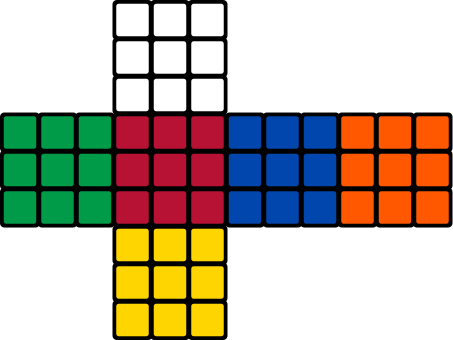
\includegraphics[width=.5\linewidth]{wiki_rubiks_colors}
	\caption{Illustration of de seks farvede sider i en 3x3 Rubiks terning.\protect\footnotemark}
\end{figure}
\footnotetext{Billede: Wikimedia Commons på \url{https://en.wikipedia.org/wiki/File:Rubik\%27s_cube_colors.svg}}
Målet er at få alle siderne til at være ens som på billedet. 
Har man selv sat sig ned med en sådan terning, virkede problemet måske meget enkelt til at starte med, men men opdager hurtigt, at det er overraskende svært.
Dette er fordi der kun er én måltilstand og et utroligt stort tilstandsrum (mere om dette senere).
Uden en algoritme vil det formentlig tage et gennemsnitligt menneske utroligt lang tid at finde en måde at løse Rubiks terning på (det tog Rubik selv en måned at komme op med en løsningsalgoritme til problemet). 
Mennesker kan spille i en time uden at lære særligt meget, men en maskine kan spille mange tusinder af spil og lære på samme måde som et menneske men på meget kortere tid. 



\section{Nyeste litteratur}
\cite{RubiksMedium}
Siden Erno Rubik opfandt sin berømte terning i 1974, er der blevet opfundet adskillige løsningsalgoritmer.
Disse kan overordnet set inddeles i to grupper:
Gruppeteoribaserede algoritmer, fx Kociembas algoritme, og brute force-algoritmer med udgangspunkt i skræddersyede heurestikker.
De forskellige algoritmer har forskellige fordele og ulemper;
nogle skal være lette for mennesker at løse, mens andre er designet til såkaldte speed cubers, der skal løse terningen med så få træk som muligt;
nogle er optimerede til lavt hukommelsesforbrug og andre til at kunne løses hurtigt af computere. 

En ny tilgang til løsningsalgoritmer og diskrete problemer generelt er dyb reinforcement learning. 


I \cite{SolvingNature} anvendes databaser af specifikke mønstre til at løse Rubiks terning. DeepCubeA formår at løse alle testkonfigurationer og generaliserer til andre diskrete spil. En korteste vej-løser er iterativt dybende A*-afsøgning med en heuristik fra Rubiks mønsterdatabase og bruger store databaser og gruppeteori. 
 
\cite{RubiksMedium} er et eksempel på anvendelse af reinforcement learning inde for kombinatorisk optimering, hvilket også inkluderer problemer såsom traveling salesman, ressource-allokering og simulering af proteinfoldning. 

\subsection{DeepCubeA}
DeepCubeA \cite{SolvingNature} kombinerer dyb læring med approksimativ værdiiteration og \emph{batch}-vægtet A*-afsøgning. Netværket ser kun ét skridt fremad, fordi at se flere skridt fremad eller anvende Monte Carlo-træafsøgning (MCTS) ikke blev fundet til at være bedre. DeepCubeA bygger på en anden implementation baseret på policy og MCTS. Den lærte kostfunktion bruges derefter som en heuristik til at finde vejen til løsningstilstanden ved brug af vægtet A*-afsøgning.  
\end{document}